\begin{center}
	\includegraphics[width=\linewidth]{images/unity_desktop.png}
\end{center}

Po zalogowaniu się do systemu ujrzysz Pulpit. Widać na nim trzy elementy --- przestrzeń roboczą, wypełniającą większą część ekranu, oraz dwa panele. Panel poziomy, zwany \textcolor{ubuntu_orange}{panelem menu}, umieszczony jest u góry ekranu. Panel pionowy to \textcolor{ubuntu_orange}{Launcher} lub inaczej panel uruchamiania, zlokalizowany z lewej strony ekranu.

\subsubsection{Zmiana tła pulpitu}
Aby zmienić tło pulpitu (inaczej: tapetę), kliknij \textbf{prawym przyciskiem myszy} wolną przestrzeń roboczą i z menu kontekstowego wybierz \textcolor{ubuntu_orange}{Zmień tło pulpitu}.

\begin{wrapfigure}{r}{0.5\textwidth}
	\vspace{-10pt}
	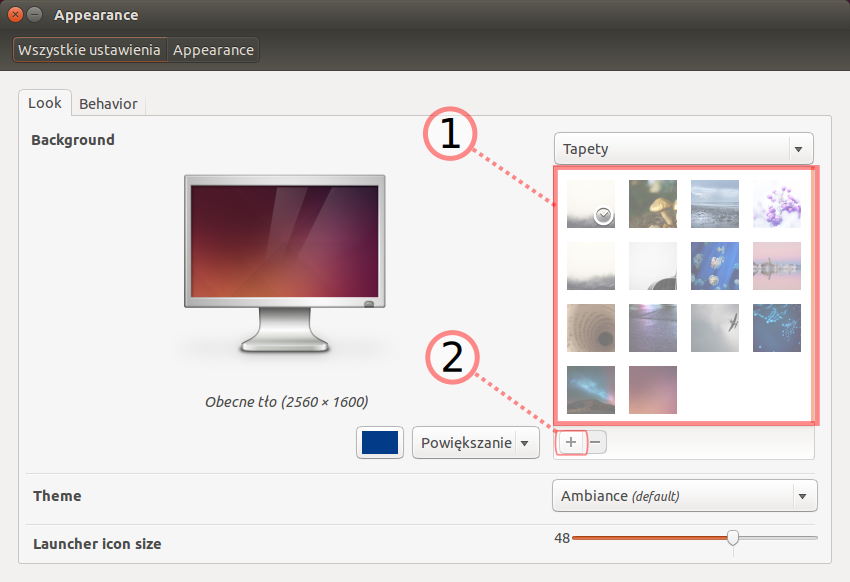
\includegraphics[width=\linewidth]{images/unity_zmiana_tapety.png}
\end{wrapfigure}

Z listy zaznaczonej jako \textcolor{ubuntu_orange}{(}1\textcolor{ubuntu_orange}{)} możesz wybrać którąś z dostępnych tapet. Kliknij przycisk plus \textcolor{ubuntu_orange}{(}2\textcolor{ubuntu_orange}{)}, aby otworzyć menadżer plików i wskazać inny plik graficzny na dysku twardym. Zostanie on użyty jako tapeta.

W tym oknie możesz też dokonać pewnych modyfikacji środowiska graficznego Unity. Zachęcamy do eksperymentów. Wszelkie zmiany są wprowadzane na żywo.
